\documentclass[conference]{IEEEtran}
\IEEEoverridecommandlockouts

\usepackage{cite}
\usepackage{amsmath,amssymb}
\usepackage{graphicx}
\usepackage{booktabs}
\usepackage{url}
\usepackage[table]{xcolor}
\usepackage{tikz}
\usetikzlibrary{arrows.meta,fit,positioning}

\definecolor{accent}{RGB}{37,99,235}
\definecolor{muted}{RGB}{150,150,150}

% Figures are generated by `python -m src.evaluation.make_figures` into docs/figures/;
% a standalone copy of this folder keeps them in figures/.
\graphicspath{{figures/}{../docs/figures/}}

\begin{document}

\title{Where Does Graph Structure Help Scholarly RAG?\\
Topical Retrieval, Citation Relatedness, and Research Discovery}

% TODO: replace with the real author list and affiliations before submission.
\author{\IEEEauthorblockN{Author names to be added}
\IEEEauthorblockA{Affiliation to be added\\
Code and artifacts: \url{https://github.com/cvishnu007/nesy-graphrag}}}

\maketitle

\begin{abstract}
Graph-based retrieval-augmented generation (GraphRAG) is increasingly proposed for scientific literature, but it is rarely tested against strong text baselines under controlled protocols. We build a neuro-symbolic literature assistant over 47,619 computer-science abstracts: neural components (dense retrieval, a local LLM, NLI, a fine-tuned entity tagger) propose, and symbolic components (a typed citation and SciERC entity graph, and rule-based provenance and citation constraints) restrict and verify what is shown. We evaluate it on four public benchmarks (SciDocs, LitSearch, DBLP, PubMed) and on project benchmarks graded by an LLM judge validated against human relevance grades ($\kappa = 0.75$ on one topic and 0.57 on ten others, where it is systematically strict; a larger judge reaches 0.88 on both). Four findings emerge. (1)~For topical queries, BM25 (0.626 NDCG@10) and BGE with BM25 (0.621) are already strong on 44 topic-stratified queries. Graph expansion adds no significant gain (0.644), even after densifying citations, because the papers it introduces are about as relevant as those they displace; a cross-encoder reranker gives a similar small gain (0.651), and a LightRAG-style entity-graph retriever scores far lower (0.396). (2)~For citation recommendation, expanding text retrieval with the papers cited by the query's nearest neighbours, an old idea, raises Recall@20 by 28\% relative ($p < 0.0001$). On DBLP and PubMed, with no training on either, it adds recall on top of every encoder tested, including the citation-trained SPECTER2 and SciNCL, and on DBLP it comes close to the trained Citeomatic system. (3)~In a time-sliced discovery benchmark, adding graph signals to text similarity nearly doubles average precision for predicting which method--task combinations appear after a cutoff. (4)~Restricting contradiction candidates to citation links raises contradiction-or-tension precision from 9\% (5 of 56) to 56\% (5 of 9) in a small single-rater study. We also report negative results: a small LLM judge distorted by batch-position bias, and graph-derived hypothesis candidates rated below a nearest-neighbour baseline by humans in two rounds. Graph structure helps scholarly RAG where the question is how papers relate, not for topical ranking.
\end{abstract}

\begin{IEEEkeywords}
retrieval-augmented generation, GraphRAG, neuro-symbolic AI, scholarly literature, citation recommendation, literature-based discovery, LLM relevance judges
\end{IEEEkeywords}

%======================================================================
\section{Introduction}

Literature-review assistants must find relevant work, surface disagreements, and suggest new directions. GraphRAG systems add a knowledge graph to retrieval on the premise that structure supplies what text similarity misses~\cite{edge2024graphrag}. For scholarly corpora the natural graphs are citations and extracted scientific entities. Whether they help is usually asserted rather than measured, and published comparisons rarely use strong text baselines, frozen development/test protocols, or validated relevance judges.

We take an empirical stance and ask: \emph{for which tasks does graph structure add value over a strong text retriever?} We contribute:
\begin{enumerate}
\item \textbf{A controlled, task-by-task evaluation} of graph structure in scholarly RAG on four public benchmarks (SciDocs, LitSearch, DBLP, PubMed) and four project benchmarks, using a dev/test protocol, pool extension, paired tests, and an LLM judge validated on human grades (Section~\ref{sec:eval}).
\item \textbf{A boundary result for graph structure.} It is redundant for topical ranking, even after densifying corpus-internal citations about $7\times$, and a LightRAG-style entity-graph retriever falls far below text retrieval (Section~\ref{sec:topical}). For citation recommendation, the neighbour-citation expansion we use is not new~\cite{strohman2007citations,bhagavatula2018content}; our contribution is showing that it still adds to modern encoders, including ones trained on citations (Sections~\ref{sec:citrec}--\ref{sec:citeomatic}). Graph signals also improve prediction of future method--task combinations (Section~\ref{sec:discovery}).
\item \textbf{A methodological warning about LLM judges.} Labels from a 3B judge agreed with a human annotator at only $\kappa = 0.19$, because of batch-position bias. Replacing them with a validated judge changed the measured effect sizes substantially (Section~\ref{sec:judge}).
\item \textbf{A neuro-symbolic assistant with human-rated reasoning modes} (Section~\ref{sec:nesy}). Citation-grounded contradiction detection works where NLI screening on abstracts did not (Section~\ref{sec:contra}). Graph-derived hypothesis candidates do not beat vector neighbours in two human rounds, and a revision chosen with an LLM judge did not transfer to held-out queries (Section~\ref{sec:hyp}).
\end{enumerate}

%======================================================================
\section{Related Work}

\textbf{GraphRAG.} Retrieval-augmented generation conditions a language model on retrieved passages~\cite{lewis2020rag}. GraphRAG~\cite{edge2024graphrag} builds LLM-extracted entity graphs with community summaries for query-focused summarisation. LightRAG~\cite{guo2025lightrag} indexes LLM-extracted entities and relations and retrieves through dual-level keyword matching; we evaluate its retrieval algorithm as a baseline. HippoRAG~\cite{gutierrez2024hipporag} runs personalised PageRank over an LLM-built graph for multi-hop QA, and HippoRAG~2~\cite{gutierrez2025hipporag2} adds deeper passage integration. Peng et al.~\cite{peng2024graphragsurvey} survey the area. Two recent studies ask our question for general corpora: Han et al.~\cite{han2025ragvsgraphrag} find RAG better on single-hop and detail questions and GraphRAG better on multi-hop reasoning, and GraphRAG-Bench~\cite{xiang2026whengraphs} finds basic RAG matching or beating GraphRAG on simple fact retrieval. These systems build their graphs with LLMs and target open-domain QA; we use citation and supervised entity graphs over scholarly text and measure, task by task, where they help.

\textbf{Neuro-symbolic AI.} Neuro-symbolic systems combine learned models with explicit symbols, rules, or structured knowledge~\cite{garcez2023neurosymbolic,kautz2022third}. Our system is a loose, pipelined coupling (the ``Neuro\,\textbar\,Symbolic'' pattern in Kautz's taxonomy): neural models propose candidates, and a typed graph and hand-written rules constrain and verify them (Section~\ref{sec:nesy}). We do not learn rules or train end to end.

\textbf{Scientific retrieval and RAG.} SPECTER~\cite{cohan2020specter}, SciNCL~\cite{ostendorff2022scincl}, and SPECTER2~\cite{singh2023scirepeval} learn citation-informed paper embeddings. OpenScholar~\cite{asai2026openscholar} retrieves over about 45 million papers. LitSearch~\cite{ajith2024litsearch} and SciDocs (introduced with SPECTER and included in BEIR~\cite{thakur2021beir}) benchmark literature search. We find that a general embedding, BGE~\cite{xiao2024cpack}, has the best NDCG@10 of the encoders tested on both public benchmarks, and that fusing it with BM25~\cite{robertson2009bm25} by reciprocal rank~\cite{cormack2009rrf} helps on LitSearch but not on SciDocs.

\textbf{Citation recommendation.} Co-citation~\cite{small1973cocitation} and bibliographic coupling~\cite{kessler1963bibliographic} are the classical citation-based relatedness measures. McNee et al.~\cite{mcnee2002citations} recommend citations by collaborative filtering over the citation graph. Strohman et al.~\cite{strohman2007citations} retrieve the papers most similar to a manuscript and add every paper they cite, which is the same expansion as our co-citation step; Citeomatic's NNSelect~\cite{bhagavatula2018content} likewise takes candidates from the query's nearest neighbours in embedding space and their citations, and then trains a reranker. ClusCite~\cite{ren2014cluscite} and Citeomatic define the DBLP and PubMed benchmarks we reuse with their published protocol. Our citation-recommendation method is therefore not new. What we add is (i)~evidence that this expansion still helps on top of modern encoders, including citation-trained ones, with no training on the target data, and (ii)~the same signal used inside a RAG assistant, where it explains each suggestion.

\textbf{Contradictions and citation function.} Citation-function analysis classifies why a paper cites another, including to criticise or contrast~\cite{teufel2006citation,jurgens2018citation,cohan2019scaffolds}. scite~\cite{nicholson2021scite} applies such a classifier to citation statements from full text at scale, labelling them supporting, contrasting, or mentioning. Our citation-grounded contradiction mode is a light, abstract-only version of the same idea: the citing sentence's critical wording is a filter rather than a trained classifier, and an LLM verdict decides. PaperQA2~\cite{skarlinski2024paperqa2} reports contradiction detection validated by experts in biology. SciFact~\cite{wadden2020scifact} provides expert-labelled claim--evidence pairs, which we use to validate verdict models.

\textbf{Literature-based discovery (LBD).} LBD predicts implicit connections from co-occurrence~\cite{swanson1986fish} and evaluates with time slicing: predictions from data before a cutoff are checked against later literature. AGATHA~\cite{sybrandt2020agatha} does this for biomedicine with graph mining and transformers, and Science4Cast~\cite{krenn2023forecasting} frames future AI research directions as link prediction in a concept network, finding hand-crafted network features strongest. SciMON~\cite{wang2024scimon} generates natural-language ideas optimised for novelty, and Si et al.~\cite{si2025ideas} find in a large blind human study that LLM-generated ideas are judged more novel but slightly less feasible than experts'. We apply the time-slicing protocol to method--task pairs extracted with a SciERC-trained tagger~\cite{luan2018scierc,beltagy2019scibert}, scored with Adamic--Adar~\cite{adamic2003friends} and citation bridges.

\textbf{Attribution and LLM judges.} ALCE~\cite{gao2023alce} evaluates citation precision and NLI support, which we adopt for answer grounding. LLMs can match human relevance labellers when the prompt is chosen against human labels~\cite{thomas2024llm}, reproduced openly as UMBRELA~\cite{upadhyay2024umbrela}, and LLM judges show position bias~\cite{zheng2023judging}, which we also observe. Agreement uses weighted kappa~\cite{cohen1968weighted}; multiple comparisons use Holm's procedure~\cite{holm1979simple}.

%======================================================================
\section{System}
\label{sec:system}

The system retrieves with three fused signals (dense, BM25, and graph expansion) over a Neo4j graph and a Chroma vector store, and four reasoning modes run on what it retrieves (Fig.~\ref{fig:arch}).

\begin{figure*}[t]
\centering
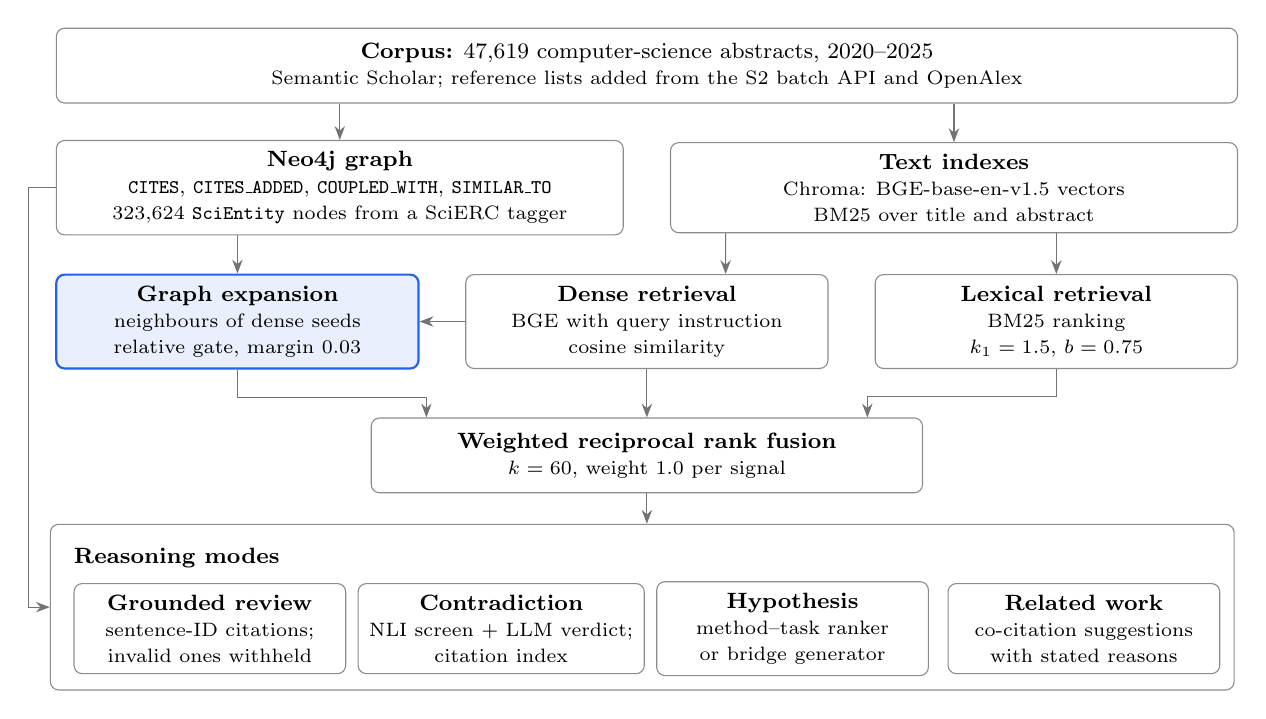
\begin{tikzpicture}[
  box/.style={draw=black!45, rounded corners=3pt, align=center, font=\footnotesize, inner sep=4pt, minimum height=0.95cm},
  acc/.style={box, draw=accent, fill=accent!10, thick},
  arr/.style={-{Stealth[length=5pt]}, draw=black!55, thin}]
\node[box, minimum width=15cm] (corpus) at (0,0)
  {\textbf{Corpus:} 47,619 computer-science abstracts, 2020--2025\\
   {\scriptsize Semantic Scholar; reference lists added from the S2 batch API and OpenAlex}};
\node[box, minimum width=7.2cm] (neo) at (-3.9,-1.55)
  {\textbf{Neo4j graph}\\
   {\scriptsize \texttt{CITES}, \texttt{CITES\_ADDED}, \texttt{COUPLED\_WITH}, \texttt{SIMILAR\_TO}}\\
   {\scriptsize 323,624 \texttt{SciEntity} nodes from a SciERC tagger}};
\node[box, minimum width=7.2cm] (idx) at (3.9,-1.55)
  {\textbf{Text indexes}\\
   {\scriptsize Chroma: BGE-base-en-v1.5 vectors}\\
   {\scriptsize BM25 over title and abstract}};
\node[acc, minimum width=4.6cm] (gexp) at (-5.2,-3.25)
  {\textbf{Graph expansion}\\
   {\scriptsize neighbours of dense seeds}\\
   {\scriptsize relative gate, margin 0.03}};
\node[box, minimum width=4.6cm] (dense) at (0,-3.25)
  {\textbf{Dense retrieval}\\
   {\scriptsize BGE with query instruction}\\
   {\scriptsize cosine similarity}};
\node[box, minimum width=4.6cm] (bm25) at (5.2,-3.25)
  {\textbf{Lexical retrieval}\\
   {\scriptsize BM25 ranking}\\
   {\scriptsize $k_1 = 1.5$, $b = 0.75$}};
\node[box, minimum width=7cm] (rrf) at (0,-4.95)
  {\textbf{Weighted reciprocal rank fusion}\\
   {\scriptsize $k = 60$, weight 1.0 per signal}};
\node[font=\footnotesize\bfseries, anchor=west] (mlabel) at (-7.4,-6.25) {Reasoning modes};
\node[box, minimum width=3.45cm] (m1) at (-5.55,-7.15)
  {\textbf{Grounded review}\\ {\scriptsize sentence-ID citations;}\\ {\scriptsize invalid ones withheld}};
\node[box, minimum width=3.45cm] (m2) at (-1.85,-7.15)
  {\textbf{Contradiction}\\ {\scriptsize NLI screen + LLM verdict;}\\ {\scriptsize citation index}};
\node[box, minimum width=3.45cm] (m3) at (1.85,-7.15)
  {\textbf{Hypothesis}\\ {\scriptsize method--task ranker}\\ {\scriptsize or bridge generator}};
\node[box, minimum width=3.45cm] (m4) at (5.55,-7.15)
  {\textbf{Related work}\\ {\scriptsize co-citation suggestions}\\ {\scriptsize with stated reasons}};
\node[draw=black!45, rounded corners=3pt, fit=(mlabel)(m1)(m2)(m3)(m4), inner sep=5pt] (modes) {};
\draw[arr] (neo.north |- corpus.south) -- (neo.north);
\draw[arr] (idx.north |- corpus.south) -- (idx.north);
\draw[arr] (gexp.north |- neo.south) -- (gexp.north);
\draw[arr] ([xshift=-2.9cm]idx.south) -- ([xshift=1.0cm]dense.north);
\draw[arr] (bm25.north |- idx.south) -- (bm25.north);
\draw[arr] (dense.west) -- (gexp.east);
\draw[arr] (gexp.south) -- ++(0,-0.35) -| ([xshift=-2.8cm]rrf.north);
\draw[arr] (dense.south) -- (rrf.north);
\draw[arr] (bm25.south) -- ++(0,-0.35) -| ([xshift=2.8cm]rrf.north);
\draw[arr] (rrf.south) -- (rrf.south |- modes.north);
\draw[arr] (neo.west) -- ++(-0.35,0) |- (modes.west);
\end{tikzpicture}
\caption{System architecture. Graph expansion (highlighted) is one of three signals fused before the reasoning modes. The left connector marks that the contradiction, hypothesis, and related-work modes also read citations and entities from the graph directly. Table~\ref{tab:nesy} lists which steps are neural and which are symbolic.}
\label{fig:arch}
\end{figure*}

\textbf{Corpus.} 47,619 Semantic Scholar~\cite{kinney2023s2} abstracts from 2020--2025 across 11 computer-science topics: artificial intelligence and machine learning, cloud computing, computer networks, computer vision, cybersecurity, data science, databases, graph neural networks, natural language processing, operating systems, and software engineering. The graph holds papers, authors, citations (\texttt{CITES}), top-5 nearest-neighbour edges (\texttt{SIMILAR\_TO}; 238,095 edges built from SPECTER vectors), and scientific entities. The language model is \texttt{qwen2.5:7b-instruct}~\cite{qwen2024qwen25}, run locally.

\textbf{Retrieval.} Three ranked lists are fused. \emph{Dense:} BGE-base-en-v1.5 over title and abstract; queries carry the BGE instruction prefix (``Represent this sentence for searching relevant passages:''). \emph{Lexical:} BM25 over title and abstract ($k_1 = 1.5$, $b = 0.75$). \emph{Graph expansion:} neighbours of the dense seeds over \texttt{CITES} and \texttt{SIMILAR\_TO} edges (up to 50 candidates). A relative gate keeps a neighbour only if its similarity to the query is at least the weakest seed's similarity minus 0.03. The lists are combined by weighted reciprocal rank fusion~\cite{cormack2009rrf}, with rank $r_s(d)$ of paper $d$ in list $s$, $k = 60$, and all weights $w_s = 1$:
\begin{equation}
\mathrm{score}(d) = \frac{1}{\sum_{s} w_s} \sum_{s \in \{\mathrm{dense},\, \mathrm{BM25},\, \mathrm{graph}\}} w_s \, \frac{k + 1}{k + r_s(d)} .
\end{equation}

\textbf{Citation densification.} Only 10,899 papers (23\%) came with reference lists, because Semantic Scholar withholds most lists for publisher-licensing reasons, and only 3.6\% of 625,222 references resolved inside the corpus. We fetched further lists from the Semantic Scholar batch API (21,027 papers) and from OpenAlex~\cite{priem2022openalex} by DOI (44,090 of 46,198 matched). The new layers use their own edge types, so the original graph and all frozen results are unchanged (Table~\ref{tab:densify}).

\begin{table}[t]
\centering
\caption{Citation graph before and after densification}
\label{tab:densify}
\resizebox{\columnwidth}{!}{%
\begin{tabular}{@{}lrr@{}}
\toprule
Graph property & Before & After \\
\midrule
Papers with a reference list & 10,899 (23\%) & 46,708 (98\%) \\
Corpus-internal citation edges & 22,370 \texttt{CITES} & + 133,527 \texttt{CITES\_ADDED} \\
Bibliographic coupling (\texttt{COUPLED\_WITH})$^{a}$ & 0 & 411,418 \\
External papers cited by $\geq 10$ corpus papers & 0 & 24,714 nodes, 641,616 edges \\
Papers with no citation link & 33,995 (71.4\%) & 6,394 (13.4\%) \\
\quad counting coupling edges & --- & 1,154 (2.4\%) \\
\bottomrule
\multicolumn{3}{@{}l}{\footnotesize $^{a}$Top 10 per paper, $\geq 2$ shared references, cosine-normalised~\cite{kessler1963bibliographic}.}
\end{tabular}}
\end{table}

\textbf{Scientific entities.} We fine-tuned SciBERT (\texttt{allenai/scibert\_scivocab\_uncased}) on the SciERC training set for 10 epochs (learning rate $5\times10^{-5}$) and kept the best development epoch (epoch 9, development F1 0.661). On the SciERC test set (100 abstracts, 1,685 gold entities), scored once, it reaches typed F1 0.639 and span F1 0.747, against 0.240 typed F1 for zero-shot GLiNER medium v2.1~\cite{zaratiana2024gliner}. Published SciBERT results on SciERC entity recognition are about 0.65--0.67. Over the corpus it extracts 1,225,433 typed mentions (Method, Task, Material, Metric, OtherScientificTerm). The graph keeps the first 15 mentions per abstract, normalised into 323,624 \texttt{SciEntity} nodes with 696,390 \texttt{MENTIONS} edges; over all mentions there are 558,123 distinct names, which the LightRAG-style baseline uses (Section~\ref{sec:topical}).

\textbf{Reasoning modes.} \emph{Grounded review:} abstracts are split into sentence passages with stable IDs; each generated claim cites passage IDs, and claims with invalid citations are withheld. \emph{Contradiction:} NLI screening with a DeBERTa-v3 cross-encoder~\cite{he2023debertav3} (\texttt{nli-deberta-v3-small}) and a structured LLM verdict over two evidence sentences, or a corpus-wide citation-grounded index (Section~\ref{sec:contra}). \emph{Hypothesis:} structural holes in the typed-entity graph, a problem-bridge generator, or a method--task ranker (Sections~\ref{sec:discovery}--\ref{sec:hyp}). \emph{Related work:} BGE + BM25 retrieval fused with co-citation suggestions, each with a stated reason.

\subsection{Neural and symbolic components}
\label{sec:nesy}

The ``neuro-symbolic'' in the project name refers to a division of labour, not to learned logic. Neural models propose; explicit structure and rules decide what is allowed and verify it (Table~\ref{tab:nesy}). This coupling is what makes outputs checkable: each answer, contradiction, or hypothesis is traceable to graph facts and passage IDs. It does not make them correct; Section~\ref{sec:grounding} shows that structurally valid citations are often not semantically supported.

\begin{table*}[t]
\centering
\caption{What is neural and what is symbolic in each step}
\label{tab:nesy}
\footnotesize
\begin{tabular}{@{}p{2.1cm}p{5.2cm}p{9.4cm}@{}}
\toprule
Step & Neural (learned) & Symbolic (explicit structure or rule) \\
\midrule
Knowledge & BGE embeddings; SciBERT--SciERC tagger extracts entities & Typed graph in Neo4j: \texttt{Paper}, \texttt{SciEntity} (Method, Task, Material, Metric, Other), \texttt{CITES}, \texttt{CITES\_ADDED}, \texttt{COUPLED\_WITH}, \texttt{MENTIONS} \\
Retrieval & Dense and BM25 ranking & Graph expansion only along typed edges, with a similarity gate; fixed RRF fusion \\
Review answers & LLM writes claims & Every claim must cite sentence-level passage IDs that exist in the retrieved set; claims with missing or unknown IDs are withheld and listed, and cited paper IDs must exist in the graph \\
Contradictions & NLI screening; LLM verdict & Candidates must be joined by a citation edge, the citing sentence must match a critical-language pattern, and both sentences must name the same specific entity \\
Hypotheses & Vector similarity between entity contexts & Only Method--Task pairs that never co-occur; Adamic--Adar over shared entities and citation links between the two sets of papers; generic-entity exclusions \\
Related work & Nearest neighbours & Suggestions come from the neighbours' citation records, shown as an explanation for each suggestion \\
\bottomrule
\end{tabular}
\end{table*}

%======================================================================
\section{Evaluation Design}
\label{sec:eval}

Every configuration is chosen on development data and tested once, every project relevance label comes from a judge validated against human grades, and every comparison reports a paired significance test with a confidence interval.

\subsection{Benchmarks}

Table~\ref{tab:bench} lists the benchmarks. The topic-stratified queries were reviewed by the team and frozen before pooling. Two near-empty queries were replaced after a corpus-support check. The retrieval configuration was frozen on 13 November 2026, and nothing was tuned on these queries. The pool is the union of the top 20 results of 8 systems. The GNN benchmark was the first project benchmark; it now serves as the judge-validation pool and is superseded for retrieval claims by the stratified set.

\begin{table*}[t]
\centering
\caption{Benchmarks}
\label{tab:bench}
\resizebox{\textwidth}{!}{%
\begin{tabular}{@{}llll@{}}
\toprule
Benchmark & Size & Documents & Labels \\
\midrule
SciDocs (BEIR) & 1,000 queries & 25,657 papers & Citation- and co-view-derived \\
LitSearch & 597 questions & 64,183 ACL/ICLR papers & Author-inspected targets \\
DBLP (Citeomatic release) & 931 test queries & 28,807 training-split candidates & Real reference lists \\
PubMed (Citeomatic release) & 8,815 test queries & 34,230 training-split candidates & Real reference lists \\
GNN project benchmark (judge validation) & 20 queries (6 dev, 14 test) & Our corpus & Validated LLM judge; 1,644 pooled pairs \\
Topic-stratified benchmark & 44 queries (4 per topic; 22 dev, 22 test) & Our corpus & Validated LLM judge; 2,305 pooled pairs \\
Citation recommendation & 600 query papers (200 dev, 400 test) & Our corpus & Real reference lists \\
Time-sliced discovery & 120 tasks, mean 4,633 candidate methods & Pre-cutoff papers (32,039) & Co-occurrence in $\geq 2$ later papers \\
SciFact (verdict models) & 338 claim--evidence pairs (122 contradictions) & Biomedical abstracts & Expert labels \\
\bottomrule
\end{tabular}}
\end{table*}

\subsection{Protocol}

\emph{Dev first, test once.} Configurations are selected on development queries, and the selection rule is written down before test results are seen. Each frozen selection runs once on test.
\emph{Pool extension.} When a new variant retrieves unjudged papers, the same blinded judge grades them, so every scored list is fully judged. We do not report condensed-list scores~\cite{sakai2007bpref} alone.
\emph{Statistics.} Paired randomisation tests: exact for up to 20 query pairs, Monte Carlo sign-flip with 20,000 samples otherwise, each with a bootstrap 95\% confidence interval. On the stratified benchmark, Holm correction~\cite{holm1979simple} covers 9 predeclared comparisons. Results near a threshold are rechecked with 1,000,000 permutations.
\emph{Metrics.} NDCG@10 is primary, with graded gain $2^g - 1$ on grades 0/1/2. Recall@20, P@10, and MAP treat grade $\geq 1$ as relevant. A unit test checks our implementations against \texttt{trec\_eval} (through \texttt{pytrec\_eval}).

\subsection{Validating the relevance judge}
\label{sec:judge}

One annotator graded a deterministic sample of 200 pooled query--paper pairs from the GNN benchmark, blinded to the method and to the AI grade. The pairs were split 50/50 by hash: judges were compared on the selection half, and the chosen judge was scored once on the held-out half. Agreement is quadratic-weighted Cohen's $\kappa$~\cite{cohen1968weighted} on the 0/1/2 scale, and the predeclared acceptance threshold was held-out $\kappa \geq 0.6$. Candidate judges were local qwen2.5 models~\cite{qwen2024qwen25} and a hosted 27B model (Table~\ref{tab:judge}).

\begin{table}[t]
\centering
\caption{Judge agreement with a human annotator (quadratic-weighted $\kappa$, GNN pairs)}
\label{tab:judge}
\resizebox{\columnwidth}{!}{%
\begin{tabular}{@{}lrr@{}}
\toprule
Judge & Selection ($n{=}100$) & Held-out ($n{=}100$) \\
\midrule
Original pool labels: qwen2.5-3B, 4 papers per call$^{a}$ & 0.166 & 0.199 \\
qwen2.5-3B, original prompt, re-run & 0.563 & 0.441 \\
qwen2.5-3B, strict prompt & 0.329 & --- \\
qwen2.5-7B, original prompt, 4 papers per call & 0.581 & --- \\
qwen2.5-7B, strict prompt, 4 papers per call & 0.602 & --- \\
\textbf{qwen2.5-7B, strict prompt, 1 paper per call (used)} & \textbf{0.769} & \textbf{0.749} \\
Qwen3.8-27B (Groq), original prompt & 0.817 & --- \\
Qwen3.8-27B (Groq), strict prompt & 0.883 & 0.884 \\
\bottomrule
\multicolumn{3}{@{}l}{\footnotesize $^{a}$0.187 on all 200 pairs.}
\end{tabular}}
\end{table}

The 27B judge is the most accurate, but the provider's free tier (200K tokens a day) covers about 200 pairs a day against about 3,950 needed. The local 7B judge, grading one paper per call, passes the threshold and graded both project pools.

\textbf{Diagnosis of the original labels.} The stored labels match the raw judge outputs exactly (0 mismatches in 1,145), so storage and alignment are not the cause. The 3B judge has a batch-position bias. Across 279 four-paper batches it used only 20 of the 81 possible grade patterns, gave the second paper a 2 in almost every batch, and produced \texttt{[0,2,2,0]} or \texttt{[0,2,0,2]} in 40\% of batches. Re-running the same model on the same pairs agreed with its own earlier labels at only $\kappa = 0.031$. Grading one paper per call raised the 7B judge's selection $\kappa$ from 0.60 to 0.77, consistent with this bias.

\textbf{Effect on conclusions.} We regraded all 1,644 pooled pairs of the GNN benchmark with the validated judge and rescored the unchanged rankings. On the 14 test queries, the selected system's lead over the original system grew from $+0.170$ ($p = 0.004$) to $+0.464$ NDCG@10 ($p = 0.0001$, 14 of 14 queries won). An apparent gap between BM25 and BGE (0.529 vs.\ 0.620) almost vanished (0.793 vs.\ 0.814). Every project retrieval number below uses the validated 7B labels.

\textbf{A second annotator and a transfer check.} A second, independent annotator graded a blinded 50-pair subset of the held-out half, stratified so that every grade is covered: human--human $\kappa = 0.91$, against 0.76--0.80 for the 7B judge and 0.86--0.95 for the 27B judge on the same pairs. Because the 200 validation pairs all come from the GNN topic, a third annotator (a project member who did not build the system; no AI assistance, blind to the judge's grades) graded 100 pairs from the other ten topics of the stratified pool, 10 per topic. There the 7B judge reaches $\kappa = 0.57$ (exact agreement 61\%, binary 74\%), below the 0.6 bar. Its errors are one-sided: it is stricter than the human on 32 items and more lenient on 7. On the sampled top-10 papers the human grades are higher by the same 0.40 for the systems with and without graph expansion, so graph comparisons are unaffected, but by 0.61 for the original system, so the gain over the original system is likely overstated and absolute NDCG values are underestimates. The 27B judge (one paper per call, temperature 0, run 20 November 2026) reaches $\kappa = 0.88$ on the same 100 pairs (exact 84\%, binary 95\%), with small two-sided errors (5 higher, 11 lower). Regrading the 2,305-pair stratified pool with it is the remaining fix.

%======================================================================
\section{Results}
\label{sec:results}

Graph structure adds nothing measurable to topical retrieval but gives large, significant gains when the target is citation-level relatedness or future method adoption. Fig.~\ref{fig:forest} summarises the paired tests.

\begin{figure*}[t]
\centering
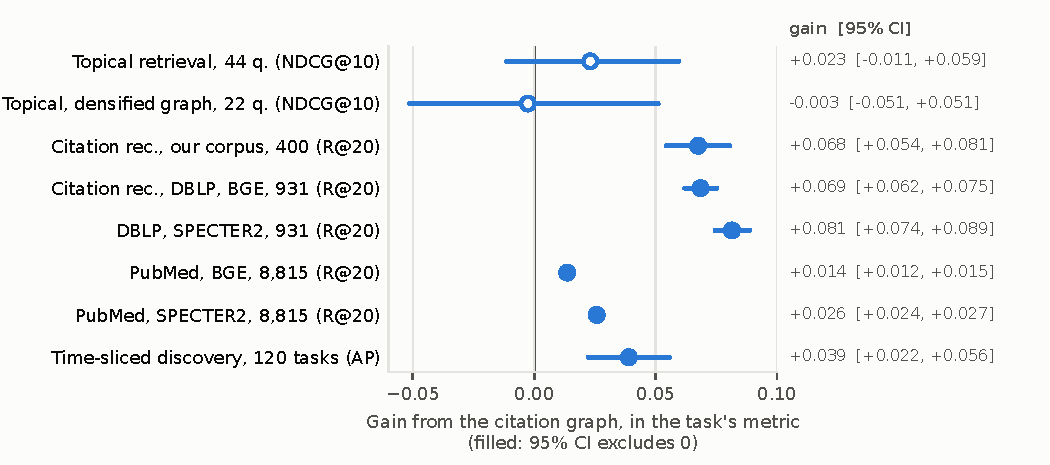
\includegraphics[width=0.92\textwidth]{fig_graph_effect.pdf}
\caption{Graph signals help citation recommendation and discovery, not topical ranking. Each row is the paired change in that task's metric when the citation graph is added to text retrieval (BGE + BM25, or the named encoder + BM25; text similarity for discovery), with a bootstrap 95\% CI. Filled markers: the CI excludes zero. Rows use different metrics, so they compare direction and significance, not magnitude.}
\label{fig:forest}
\end{figure*}

\subsection{Retrieval models on public benchmarks}

BGE has the highest NDCG@10 of all embeddings on both benchmarks (Table~\ref{tab:public}); on SciDocs, MiniLM (0.510) and SciNCL (0.508) have higher Recall@100 than BGE (0.493). Every alternative beats SPECTER on LitSearch ($p \leq 0.013$), and BGE beats OpenScholar's retriever by 0.055 on SciDocs and 0.172 on LitSearch (both $p < 0.001$). BM25 fusion improves every dense model on LitSearch's natural-language questions, but lowers BGE and MiniLM on SciDocs, whose queries are paper titles. Our SciDocs scores are close to published BEIR values (MiniLM 0.217 vs.\ 0.216; BM25 0.152 vs.\ 0.158). SPECTER2 was run without its task adapters, so its scores are a lower bound.

\begin{table}[t]
\centering
\caption{NDCG@10 on public benchmarks, alone and fused with BM25}
\label{tab:public}
\resizebox{\columnwidth}{!}{%
\begin{tabular}{@{}lrrrr@{}}
\toprule
Embedding & SciDocs & + BM25 & LitSearch & + BM25 \\
\midrule
BGE-base-en-v1.5 (general) & \textbf{0.218} & 0.198 & \textbf{0.449} & \textbf{0.489} \\
MiniLM-L6-v2 (general) & 0.217 & 0.198 & 0.352 & 0.456 \\
SciNCL & 0.196 & \textbf{0.199} & 0.241 & 0.393 \\
SPECTER2 base, no adapter & 0.172 & 0.185 & 0.331 & 0.462 \\
OpenScholar retriever & 0.163 & 0.177 & 0.277 & 0.410 \\
SPECTER (original system) & 0.151 & 0.180 & 0.208 & 0.377 \\
BM25 alone & 0.152 & --- & 0.395 & --- \\
\bottomrule
\end{tabular}}
\end{table}

\subsection{Topical retrieval: graph structure is redundant}
\label{sec:topical}

The selected system wins 40 of 44 queries against the original system (Tables~\ref{tab:strat} and~\ref{tab:stratcmp}). Its advantage over BGE alone ($+0.052$) is not significant after Holm correction ($p = 0.0104$ with 1,000,000 permutations under two seeds; the 20,000-permutation estimate, 0.0095, had fallen within sampling error of the threshold); most of it comes with BM25 fusion. Graph expansion over BGE + BM25 adds a non-significant $+0.023$, and graph expansion alone does not help BGE. BM25 is a strong baseline on this corpus, and the selected system's lead over it is not significant. On the 14 GNN test queries the picture is the same: the selected system (0.813) ties BGE alone (0.814; $p = 0.96$). The gap to the original system ($+0.358$) is real but likely overstated, because the judge under-grades the original system's papers more than ours (Section~\ref{sec:judge}).

\begin{table}[t]
\centering
\caption{Topic-stratified benchmark, 44 queries}
\label{tab:strat}
\resizebox{\columnwidth}{!}{%
\begin{tabular}{@{}lrrr@{}}
\toprule
System & NDCG@10 & P@10 & Recall@20 \\
\midrule
\textbf{BGE + BM25 + graph (selected)} & \textbf{0.644} & \textbf{0.725} & \textbf{0.613} \\
BM25 & 0.626 & 0.691 & 0.534 \\
BGE + BM25 & 0.621 & 0.702 & 0.588 \\
BGE & 0.593 & 0.684 & 0.556 \\
BGE + graph & 0.585 & 0.680 & 0.589 \\
Original system (SPECTER, absolute gate) & 0.287 & 0.382 & 0.264 \\
\bottomrule
\end{tabular}}
\end{table}

\begin{table}[t]
\centering
\caption{The nine predeclared comparisons on the 44 stratified queries ($\Delta$ NDCG@10; $p$ from 1,000,000 sign-flip permutations)}
\label{tab:stratcmp}
\resizebox{\columnwidth}{!}{%
\begin{tabular}{@{}lrlrr@{}}
\toprule
Comparison & $\Delta$ & 95\% CI & $p$ & Holm-adj. \\
\midrule
Selected vs.\ original system & $+0.358$ & [$0.285$, $0.434$] & $<0.0001$ & $<0.0001$ \\
BM25 vs.\ original system & $+0.339$ & [$0.270$, $0.406$] & $<0.0001$ & $<0.0001$ \\
BGE + BM25 vs.\ original system & $+0.334$ & [$0.265$, $0.405$] & $<0.0001$ & $<0.0001$ \\
BGE vs.\ original system & $+0.306$ & [$0.235$, $0.381$] & $<0.0001$ & $<0.0001$ \\
Selected vs.\ BGE & $+0.052$ & [$0.012$, $0.087$] & 0.0104 & 0.052 \\
Selected vs.\ BGE + BM25 (graph) & $+0.023$ & [$-0.011$, $0.059$] & 0.21 & 0.84 \\
Selected vs.\ BM25 & $+0.019$ & [$-0.029$, $0.064$] & 0.45 & 0.90 \\
BGE vs.\ BM25 & $-0.033$ & [$-0.090$, $0.024$] & 0.27 & 0.84 \\
BGE + graph vs.\ BGE & $-0.008$ & [$-0.053$, $0.034$] & 0.74 & 0.90 \\
\bottomrule
\end{tabular}}
\end{table}

\textbf{Densified graph.} We reran graph expansion with the densified layers, chose the best of three dense variants on the 22 development queries (\texttt{CITES} + \texttt{CITES\_ADDED} + \texttt{COUPLED\_WITH}, NDCG@10 0.693), and tested it once on the 22 test queries. Against no graph it scored $-0.003$ (0.540 vs.\ 0.543; $p = 0.92$), and against the current graph $-0.036$ ($p = 0.20$). Recall@20 rose slightly (0.605 vs.\ 0.585 without a graph).

The denser graph finds equally relevant alternatives, not better ones. On the development queries, the 63 papers that dense expansion moved into the top 10 have the same mean relevance as the 63 they displaced (1.19 vs.\ 1.21 on the 0--2 scale; 51\% grade 2 in both). BGE + BM25 already fills the top 10 with relevant papers (P@10 $\approx 0.78$), so swaps cannot raise the score.

\textbf{Reranker baseline.} A cross-encoder reranker is the standard alternative to graph expansion. Reranking the top 20 of BGE + BM25 with \texttt{ms-marco-MiniLM-L-6-v2} (depth 20 is the judged pool depth, so the reranked top 10 needs no new labels; titles and abstracts from the Semantic Scholar API) gives 0.651 ($+0.030$ [$-0.004$, $0.066$], $p = 0.11$), about the same as graph expansion and not distinguishable from it ($+0.007$, $p = 0.78$). Reranking the graph-expanded list gives 0.668, not significantly above either ($+0.023$ over the selected system, $p = 0.34$). Fig.~\ref{fig:topical} shows all systems with bootstrap intervals.

\begin{figure*}[t]
\centering
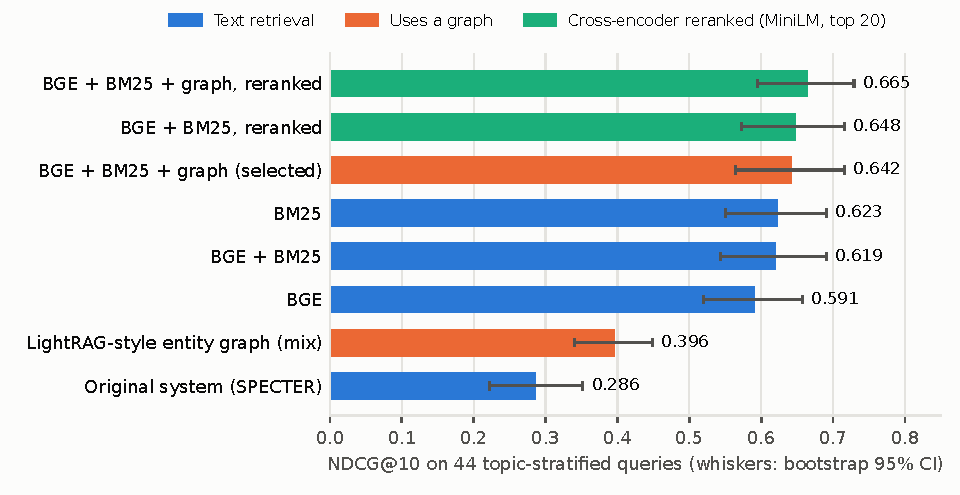
\includegraphics[width=0.82\textwidth]{fig_topical_ndcg.pdf}
\caption{Topical retrieval on 44 stratified queries. Text retrieval, graph expansion, and a small cross-encoder reranker are within each other's confidence intervals; the LightRAG-style entity-graph retriever and the original system are far lower. Scored with the extended pool (3,073 pairs) so that every system shown is fully judged; the selected system scores 0.642 here and 0.644 on the original pool.}
\label{fig:topical}
\end{figure*}

\textbf{GraphRAG baseline.} A real LightRAG index needs about two LLM extraction calls per chunk, more than a week for 47,619 abstracts on our 4\,GB laptop GPU. We therefore keep LightRAG's query-time algorithm~\cite{guo2025lightrag} and replace only its LLM-built index with the SciERC graph: 558,123 entities embedded by name with BGE, and 604,108 relations (entity pairs co-occurring in at least 2 abstracts). The local 7B model extracts high- and low-level keywords with LightRAG's instructions. In its default mix mode (a round-robin of BGE, entity, and relation retrieval) it reaches 0.396 NDCG@10, and 0.176 in hybrid mode, against 0.642 for our system on the same extended pool ($+0.246$, 39 wins and 3 losses, $p < 0.0001$) and 0.591 for BGE alone. Entity-centric retrieval ranks papers by which entities they mention, not by whether they address the query: the 7B model's low-level keywords are often generic (``scalability'', ``resource allocation'') and match entities found in thousands of papers. This is a re-implementation over a supervised graph, not the original package, and a stronger LLM might narrow the gap.

\subsection{Citation recommendation: graph structure helps}
\label{sec:citrec}

Given a corpus paper's title and abstract, the task is to rank the corpus papers it cites. Ground truth is the real reference lists (\texttt{CITES} + \texttt{CITES\_ADDED}), with no LLM judge. Three leakage controls apply: the query paper's own citation edges are never used; papers that cite the query paper are excluded from the neighbour set; and every method ranks only papers published no later than the query paper.

The graph signal is neighbour co-citation: papers cited by the query's $k$ nearest BGE neighbours, weighted by neighbour similarity. Of 9,534 eligible papers (published 2022 or later, citing $\geq 5$ older corpus papers), 600 were selected by hash. Settings were chosen on dev by Recall@20 from a predeclared grid ($k \in \{10, 20, 50\}$, weight $\in \{0.5, 1.0\}$). The chosen setting, $k = 50$ with weight 1.0, lies at the edge of the grid and ran once on test.

\begin{table}[t]
\centering
\caption{Citation recommendation, 400 test papers}
\label{tab:citrec}
\resizebox{\columnwidth}{!}{%
\begin{tabular}{@{}lrrr@{}}
\toprule
Method & Recall@20 & NDCG@10 & MAP \\
\midrule
\textbf{BGE + BM25 + co-citation graph} & \textbf{0.308} & \textbf{0.283} & \textbf{0.188} \\
Co-citation graph alone & 0.267 & 0.250 & 0.159 \\
BGE & 0.251 & 0.231 & 0.142 \\
BGE + BM25 & 0.241 & 0.217 & 0.135 \\
BM25 & 0.169 & 0.155 & 0.091 \\
\bottomrule
\end{tabular}}
\end{table}

Adding the graph to BGE + BM25 raises Recall@20 by $+0.068$ (95\% CI [0.055, 0.081], $p < 0.0001$), 28\% relative, and NDCG@10 by $+0.067$ (Table~\ref{tab:citrec}). Over BGE alone the gain is $+0.057$ Recall@20 ([0.043, 0.072], $p < 0.0001$). The graph alone does not significantly beat BGE ($+0.016$, $p = 0.17$), so the two signals are complementary. Development results agree ($+0.071$ Recall@20 over BGE + BM25). Unlike topical retrieval, BM25 fusion slightly hurts here, where queries are long abstracts.

\subsection{Citation recommendation on DBLP and PubMed}
\label{sec:citeomatic}

On the DBLP and PubMed benchmarks of Bhagavatula et al.~\cite{bhagavatula2018content}, we run the same method, with no training on either dataset, under the published protocol: splits by year, candidates from the training split only, gold references that are older, in-corpus training papers (queries need at least 10), F1@20 as the harmonic mean of corpus-level P@20 and R@20, and MRR over the top 100. The expansion is close to Citeomatic's NNSelect candidate step, so this tests whether an old idea still adds to modern encoders, not a new method (Table~\ref{tab:citeomatic}).

\begin{table}[t]
\centering
\caption{DBLP and PubMed test splits (F1@20 / MRR); bold: best of our methods}
\label{tab:citeomatic}
\resizebox{\columnwidth}{!}{%
\begin{tabular}{@{}lll@{}}
\toprule
Method & DBLP & PubMed \\
\midrule
BGE + BM25 & 0.230 / 0.649 & 0.290 / 0.747 \\
BGE + BM25 + co-citation & 0.284 / 0.677 & 0.305 / 0.699 \\
SPECTER2 + BM25 & 0.236 / 0.663 & 0.288 / \textbf{0.748} \\
SPECTER2 + BM25 + co-citation & \textbf{0.300} / \textbf{0.708} & \textbf{0.316} / 0.724 \\
SciNCL + BM25 & 0.230 / 0.629 & 0.270 / 0.719 \\
SciNCL + BM25 + co-citation & 0.283 / 0.666 & 0.281 / 0.663 \\
\midrule
ClusCite (published) & 0.237 / 0.548 & 0.274 / 0.578 \\
Citeomatic NNSelect (published) & 0.282 / 0.579 & 0.309 / 0.699 \\
Citeomatic, best (published) & 0.303 / 0.689 & 0.329 / 0.771 \\
\bottomrule
\end{tabular}}
\end{table}

On DBLP, co-citation adds $+0.069$ Recall@20 and $+0.028$ MRR over BGE + BM25 (both significant) and comes close to the trained Citeomatic system. The gain is not specific to BGE: co-citation adds $+0.069$ to $+0.081$ Recall@20 on top of all three encoders ($p < 0.001$), and SPECTER2 + BM25 + co-citation reaches 0.300 F1@20 and 0.708 MRR, against 0.303 and 0.689 for Citeomatic. So, on DBLP, the citation graph carries information that these citation-trained embeddings do not already capture. Two caveats apply: SPECTER2 and SciNCL were pretrained on citation links from Semantic Scholar, which probably include many DBLP and PubMed papers, so they are not training-free; and the comparison is with 2018 systems. On PubMed co-citation adds $+0.010$ to $+0.026$ Recall@20 across the three encoders but lowers MRR by 0.023 (SPECTER2) to 0.056 (SciNCL). A diagnosis on the validation year shows why: co-citation favours widely cited papers in both datasets, but on PubMed text retrieval already ranks a correct paper first 71\% of the time against 45\% for the graph alone, so equal-weight fusion displaces correct first picks; on DBLP the two are equally precise at the top (52\%).

\subsection{Time-sliced discovery: graph signals predict future research}
\label{sec:discovery}

A hypothesis is ``method $M$ could be applied to task $T$'' for a SciERC (Task, Method) pair that never co-occurs in any paper up to the 2022 cutoff. It is confirmed if the pair co-occurs in $\geq 2$ later papers. Scorers see only the 32,039 pre-cutoff papers, with their entities, BGE vectors, and citations among themselves; entity frequencies and the generic-entity filter are recomputed on those papers. The benchmark has 120 tasks with $\geq 10$ pre-cutoff papers and $\geq 3$ confirmed methods, with on average 4,633 candidate methods and 5.6 confirmed methods per task. Scorers were predeclared and nothing was tuned.

\begin{table}[t]
\centering
\caption{Time-sliced discovery, 120 tasks (cutoff 2022)}
\label{tab:temporal}
\resizebox{\columnwidth}{!}{%
\begin{tabular}{@{}lrrrr@{}}
\toprule
Scorer & AP & P@10 & R@100 & AUROC \\
\midrule
Fusion: popularity + vector + entity + citation & \textbf{0.087} & 0.066 & \textbf{0.441} & \textbf{0.927} \\
\textbf{Fusion: vector + entity graph + citation graph} & 0.083 & \textbf{0.067} & 0.406 & 0.894 \\
Fusion: entity graph + citation graph & 0.077 & 0.063 & 0.390 & 0.864 \\
Entity-graph bridge (Adamic--Adar) & 0.072 & 0.061 & 0.398 & 0.860 \\
Vector similarity (text only) & 0.044 & 0.037 & 0.302 & 0.846 \\
Popularity & 0.032 & 0.023 & 0.288 & 0.896 \\
Citation-graph bridge & 0.017 & 0.011 & 0.231 & 0.679 \\
Random & 0.003 & 0.003 & 0.024 & 0.506 \\
\bottomrule
\end{tabular}}
\end{table}

Adding graph signals to text similarity raises AP by $+0.039$ (95\% CI [0.022, 0.056], $p < 0.0001$) and Recall@100 by $+0.103$ (Table~\ref{tab:temporal}). The graph signals alone also beat text ($+0.033$ AP, $p = 0.0004$). The result holds on the 60-task test half ($+0.043$, $p = 0.003$), with a 2021 cutoff (135 tasks; 0.142 vs.\ 0.097, $p < 0.0001$), and with a stricter $\geq 3$ confirming papers (32 tasks; 0.079 vs.\ 0.043, $p = 0.035$). The citation bridge is weak alone but complements the entity graph.

\textbf{From scores to generators.} Each arm proposes 10 methods per task from pre-cutoff data. Ranking (task, method) pairs directly with the vector + graph scorer reaches P@10 0.067, against 0.038 for the methods of vector-neighbour papers (the baseline in our human study) and 0.023 for popularity. A paper-candidate bridge generator, which proposes only methods that none of the 15 nearest papers mention, reaches 0.021, below the vector-neighbour baseline ($-0.017$, 95\% CI [$-0.033$, $-0.001$], $p = 0.053$). Its novelty filter discards the methods researchers most often adopt next. In the full application the ranker filters generic heads (``X methods'') and task acronyms of 3 characters or fewer; with that filter the advantage holds (94 tasks; P@10 0.052 vs.\ 0.028, $p < 0.0001$).

\subsection{Hypothesis candidates rated by humans}
\label{sec:hyp}

\textbf{Round 1.} For each of 30 stratified queries, two raters saw the top structural-hole candidate from the entity graph and a vector-neighbour baseline (vector rank 6--15, not cited by the top 5), shuffled and blinded. Inter-rater $\kappa$ is 0.90 for relevance, 0.82 for novelty, and 0.89 for promise. Ratings are averaged over raters and paired by query, with a Monte Carlo sign-flip test (Table~\ref{tab:hyp}). The structural-hole candidates are significantly less relevant and less promising, and no more novel. The rater notes (``unrelated: IDS survey'', ``generic gnn tutorial'') trace this to links through broad shared concepts. Round 1 ran with the generic-entity filter off (the code default at the time); with it on, 21 of the 30 top candidates change.

\begin{table}[t]
\centering
\caption{Human ratings of hypothesis candidates, round 1 (1--5, 30 queries, mean of two raters)}
\label{tab:hyp}
\resizebox{\columnwidth}{!}{%
\begin{tabular}{@{}lrrlr@{}}
\toprule
Rating & Structural hole & Vector neighbour & Graph $-$ vector [95\% CI] & $p$ \\
\midrule
Relevance & 3.10 & \textbf{4.12} & $-1.02$ [$-1.50$, $-0.52$] & \textbf{0.001} \\
Novelty & 1.88 & 2.17 & $-0.28$ [$-0.67$, 0.10] & 0.20 \\
Promise & 2.15 & \textbf{2.67} & $-0.52$ [$-0.93$, $-0.10$] & \textbf{0.03} \\
\bottomrule
\end{tabular}}
\end{table}

\textbf{Revision and round 2.} A problem-bridge generator follows the LBD pattern ``apply method $M$ to problem $T$'': a candidate must share a specific Task or Material entity (IDF-weighted) with the query papers, mention a Method that none of the 15 nearest papers mention, stay above a relevance floor, and lie outside the vector top 15. On the round-1 queries the validated 7B judge preferred it (mean relevance 0.77 on 0--2, against 0.43 for the original structural hole). Round 2 tested it on the 14 held-out stratified queries with four blinded arms and the generic filter on, rated by one rater (Table~\ref{tab:hyp2}). The bridge was no better than the original and did not beat vector neighbours (relevance 3.54 vs.\ 3.93, promise 3.31 vs.\ 3.64; not significant with 13 pairs). The original again scored lower on promise (3.00 vs.\ 3.64, $p = 0.03$). Paper-level graph candidates thus lose to vector similarity in both rounds; only the method--task ranker (Section~\ref{sec:discovery}) shows a graph advantage, on the time-sliced benchmark.

\begin{table}[t]
\centering
\caption{Round 2: held-out queries, four arms, one rater (1--5)}
\label{tab:hyp2}
\resizebox{\columnwidth}{!}{%
\begin{tabular}{@{}lrrrr@{}}
\toprule
Arm & $n$ & Relevance & Novelty & Promise \\
\midrule
Vector neighbour & 14 & \textbf{3.93} & 2.86 & \textbf{3.64} \\
Original structural hole & 14 & 3.50 & 2.36 & 3.00 \\
Problem bridge (selected on dev) & 13 & 3.54 & 2.77 & 3.31 \\
Problem bridge, specific entities only & 13 & 3.54 & 2.92 & 3.31 \\
\bottomrule
\end{tabular}}
\end{table}

\subsection{Contradictions}
\label{sec:contra}

\textbf{Verdict models on SciFact.} We ran the application's structured prompt, without tuning, on 338 expert-labelled SciFact pairs (122 contradictions; Table~\ref{tab:verdict}). GPT-OSS-120B~\cite{openai2025gptoss} answered 337 of 338 items before the provider's daily token limit; the missing item is a non-contradiction, and the worst-case F1 is 0.809. The 3B model labels 264 of 338 pairs as contradictions, falling below the 0.64 majority baseline in accuracy, and gives confidence 1.0 to every verdict. We therefore screen with NLI locally and take verdicts from a larger model.

\begin{table}[t]
\centering
\caption{Contradiction verdicts on SciFact (338 pairs)}
\label{tab:verdict}
\resizebox{\columnwidth}{!}{%
\begin{tabular}{@{}lrrrrr@{}}
\toprule
Verdict model & Prec. & Recall & F1 & Acc. & ECE \\
\midrule
qwen2.5-3B-instruct (local) & 0.386 & 0.836 & 0.528 & 0.462 & 0.538 \\
qwen2.5-7B-instruct (local) & 0.849 & 0.598 & 0.702 & 0.817 & --- \\
Qwen3.8-27B (Groq) & 0.953 & 0.672 & 0.788 & 0.870 & 0.089 \\
\textbf{GPT-OSS-120B (Groq)} & 0.946 & 0.713 & \textbf{0.813} & \textbf{0.881} & \textbf{0.066} \\
NLI screening alone (dev threshold) & 0.614 & 0.730 & 0.667 & 0.737 & --- \\
\bottomrule
\multicolumn{6}{@{}l}{\footnotesize NLI screening AUROC: 0.818.}
\end{tabular}}
\end{table}

\textbf{In-corpus contradictions, round 1.} Two raters ($\kappa = 0.76$) labelled 68 pairs from the NLI sentence-pair screener (30 stratified queries, top 20 retrieved papers each): 56 top-ranked candidates and 12 lower-ranked controls. No pair is a contradiction for both raters. One rater called 2 of the 56 top pairs contradictions (both on LLM-based versus search-based unit-test generation) and the other called them tensions; 7 of 56 (12.5\%) are a tension or contradiction for at least one rater, against 0 of 12 controls. The screener mostly pairs papers that each report their own gains. A 7B verdict filter cuts the pairs shown from 68 to 5: it keeps both disputed pairs, and the other 3 (about 5\% of negatives) are false alarms.

\textbf{Revision: a citation-grounded index.} Disagreements in computer science are usually written on purpose, in replications, ``revisiting'' papers, and negative results, and the disputing paper cites the disputed one. The index pairs critical findings (``fails to'', ``contrary to'', ``surprisingly'') with the papers they cite, requires a shared specific SciERC entity in both sentences, and ranks pairs by NLI. On the densified graph it finds 591 candidates; the 7B verdict model flags 9 of the top 150. In round 2, one rater (the system's developer) labelled 40 blinded pairs: 5 of the 9 verdict-flagged pairs (56\%; 95\% Wilson CI 27--81\%) are a contradiction or tension, including 2 real contradictions (a follow-up reporting that Post2Vec does not improve over the state of the art; constructive exact low-rank embeddings against an impossibility result). The same rater labelled 9\% (5 of 56) of the round-1 screener's top pairs as tensions and none as contradictions (Fisher $p = 0.003$ and $0.017$). Round 1 and round 2 use different queries and pair sources, so this comparison is indicative, and the 56\% rests on 9 pairs. NLI rank within the index matters (top 150: 10 of 24 vs.\ rank 151+: 1 of 16, $p = 0.03$); the verdict filter's extra gain (56\% vs.\ 33\%) is not significant at this size.

\subsection{Answer grounding}
\label{sec:grounding}

We compared standard vector RAG (BGE) with our system (BGE + BM25 + graph) at a matched budget: the same generator and prompt, top 5 papers, a 6,000-character evidence budget, and no repair attempts. A claim counts as supported if a local NLI model (\texttt{cross-encoder/nli-deberta-v3-small}, confidence $\geq 0.5$) finds it entailed by the passages it cites (Table~\ref{tab:grounding}).

\begin{table}[t]
\centering
\caption{Answer grounding at a matched budget}
\label{tab:grounding}
\resizebox{\columnwidth}{!}{%
\begin{tabular}{@{}lrrrr@{}}
\toprule
 & \multicolumn{2}{c}{3B, 14 GNN test queries} & \multicolumn{2}{c}{7B, 44 stratified queries} \\
\cmidrule(lr){2-3}\cmidrule(lr){4-5}
 & Vector RAG & Our system & Vector RAG & Our system \\
\midrule
Claims per answer & 5.79 & 5.93 & 3.57 & 3.59 \\
Structural citation precision & 0.984 & 0.995 & 1.000 & 0.998 \\
\textbf{Claims supported by cited passages} & \textbf{0.321} & \textbf{0.277} & \textbf{0.389} & \textbf{0.418} \\
Claims contradicted by cited passages & 0.062 & 0.120 & 0.038 & 0.070 \\
\bottomrule
\end{tabular}}
\end{table}

Neither comparison is significant. The per-query support difference (our system $-$ vector RAG) is $-0.043$ with the 3B generator (95\% CI [$-0.248$, 0.150], exact $p = 0.69$) and $+0.046$ with the 7B generator ([$-0.068$, 0.157], $p = 0.43$). Support is higher with the 7B generator, but the two runs used different queries, so that change is only indicative. In both, nearly all citations are structurally valid, yet about 60\% or more of claims are not entailed by the passages they cite. Passage-ID validation alone therefore overstates grounding, and semantic support checks are needed. NLI support is an automated proxy that still awaits human validation.

%======================================================================
\section{Discussion}

\textbf{Topical retrieval for short queries saturates with text.} BGE + BM25 already places relevant papers in most of the top 10, so graph expansion can only swap them for equally relevant ones (1.19 vs.\ 1.21 mean grade), and a cross-encoder reranker gains about as much. This agrees with GraphRAG-Bench~\cite{xiang2026whengraphs} and Han et al.~\cite{han2025ragvsgraphrag} on general corpora. Retrieving through entities instead of text loses relevance, because a paper's entities say little about whether it addresses the query.

\textbf{Citation structure carries different information.} When the target is citation-level relatedness or future method adoption, which is what ``who builds on whom'' encodes, graph signals add large, significant gains, and they complement text: co-citation alone does not beat BGE significantly, but fusing the two does, on our corpus and on DBLP. In biomedicine the gain in recall comes with a loss at the top of the ranking, where text is already very precise.

\textbf{How a signal is used matters.} The same entity graph that predicts future method--task combinations (Section~\ref{sec:discovery}) produced weak hypotheses when it was routed through candidate papers with a novelty filter (Sections~\ref{sec:discovery}--\ref{sec:hyp}). Ranking (task, method) pairs directly preserves the signal.

\textbf{Disagreement is written into citations.} In computer-science abstracts, contradictions are rare between topically similar papers but appear where one paper explicitly revisits another; restricting candidates to citation links is what made the contradiction mode useful (Section~\ref{sec:contra}).

\textbf{Judges must be validated, and LLM-judge selection can overfit.} An unvalidated 3B judge would have reported a $+0.170$ gain over the original system where a validated judge measures $+0.464$, and a judge validated on one topic proved too strict on others. The hypothesis revision chosen with the 7B judge on development queries did not beat the baseline for a human on held-out queries (Section~\ref{sec:hyp}), so human test sets remain necessary for generative modes.

%======================================================================
\section{Limitations}

\begin{itemize}
\item Abstracts only, from one corpus: computer science, 2020--2025, 47,619 papers. Results may differ with full text or other fields.
\item Public citation benchmarks: the published comparison systems are from 2018, and our modern baselines are encoders (BGE, SPECTER2, SciNCL), not trained citation recommenders. The encoders' training data likely overlap with DBLP and PubMed papers. The citation-graph benefit does not transfer fully to biomedicine (PubMed MRR drops).
\item The GraphRAG baseline re-implements LightRAG's retrieval over our SciERC graph; the original LLM-built index (and Microsoft GraphRAG) was infeasible at this scale on our hardware, and a stronger LLM might narrow the gap.
\item Missing baselines: no Personalized-PageRank graph retriever in the style of HippoRAG~2, no learned link predictor for the time-sliced benchmark (Science4Cast found such models competitive), and the reranker uses a small model at depth 20 rather than a larger model at depth 50--100. SPECTER2 was evaluated without its adapters.
\item Project relevance labels come from an LLM judge (held-out $\kappa = 0.75$ against the first annotator). On the other ten topics of the stratified benchmark it agrees less with a human ($\kappa = 0.57$) and is systematically strict; this does not bias graph comparisons but likely inflates the gain over the original system. Human--human agreement was measured on only 50 pairs ($\kappa = 0.91$).
\item Raters are anonymous and identified by role. Rater A, on every human task, is a project member who built the system, although every sheet was blind to method. Round 2 has only Rater A. Raters B and C are project members who did not build the system; their independence (no AI, no access to Rater A's sheets) was confirmed by the project owner but not recorded under a formal protocol.
\item Two leakage paths are not yet closed in the frozen runs: in citation recommendation, near-duplicate versions of a query paper (51 pairs in the corpus, cosine $\geq 0.995$) can be among its neighbours; in the time-sliced benchmark, entity types are decided from all mentions, including post-cutoff ones. Fixes exist as options but have not been run.
\item Per-query results were not saved for citation recommendation, DBLP/PubMed, and the time-sliced benchmark, so their means and tests can be checked against saved summaries but not recomputed without rerunning.
\item ``Confirmed'' in the time-sliced benchmark means co-occurrence in later abstracts, not a successful result, and it misses combinations described in other words. Entities come from an automatic extractor (typed F1 0.64). Hypotheses described as ``never combined in the corpus'' may already exist in older literature.
\item SciFact is biomedical, so the verdict models are validated off-domain; in-corpus contradiction precision rests on small human samples (68 pairs with two raters, 40 with one), and the round-2 headline on 9 pairs.
\item Answer grounding is scored by a small NLI model without a human check of its support labels.
\item Three points deviate from our written protocol: hypotheses were rated on three 1--5 scales instead of a five-dimension rubric; the contradiction evaluation has at most 2 confirmed contradictions per arm, not 10 positives per split; and the judge-transfer check used one rater. The neuro-symbolic coupling is rule-based and hand-written, and rules such as the critical-language pattern were designed on this corpus.
\end{itemize}

%======================================================================
\section{Conclusion}

Graph structure is not a general upgrade for scholarly RAG. On 47,619 computer-science abstracts it is redundant for topical ranking, even after a $7\times$ densification of citations, but it adds substantial value for citation recommendation ($+28\%$ Recall@20 on our corpus, with consistent gains on DBLP) and research discovery (nearly $2\times$ average precision). Evaluations of GraphRAG should name the task, compare against strong text baselines including BM25 fusion and reranking, and validate their relevance judges against human grades on every topic they cover.

\textbf{Future work.} Regrading the stratified pool with the 27B judge; closing the two leakage paths and saving per-query results; a second rater for round 2 and more labelled contradiction pairs; the missing baselines listed above; and a study of how the graph's value changes as the corpus grows.

\textbf{Reproducibility.} Code, configurations, frozen query sets, judge prompts, human-label sheets, and result artifacts are in the repository (\texttt{src/evaluation/}, \texttt{results/}, \texttt{evaluation/}). The command \texttt{python -m src.evaluation.reproduce} checks 35 headline numbers without LLM calls or databases and fails if any differs from its reported value by more than 0.0015: 26 are recomputed from raw rankings, labels, and rating sheets (the hidden annotator keys are rebuilt from the kits' fixed seeds), and 9 are read from saved summaries until per-query files exist. Data licences: Semantic Scholar abstracts (ODC-By), OpenAlex (CC0), SciFact (claims and annotations CC BY 4.0; abstracts ODC-By 1.0); LitSearch, SciDocs, DBLP, and PubMed under their own terms.

\bibliographystyle{IEEEtran}
\bibliography{references}

\end{document}
